\section{The Machine Learning Models}
For every prediction of the hessian matrix, it is necessary to use the homonuclear and heteronuclear model.
Both models were further investigated by three adjustments, namely the algorithms, the labeling and a generalization.\\
At first, as described in the Chapter Theory, the RFR and ETR are used as the different algorithms for the fitting of the ML model.
For the labeling the two possible cases of the labeling, which are the indexed and permuted case were discussed.
At last, it is investigated, how the performance changes if instead of fitting the ML model only case--specific
the ML model is fitted to a general model, that predicts all cases.

\section{The $\mathrm{\textbf{H}}_\mathrm{\textbf{2}}$ system}
\begin{figure}[H]
    \centering
    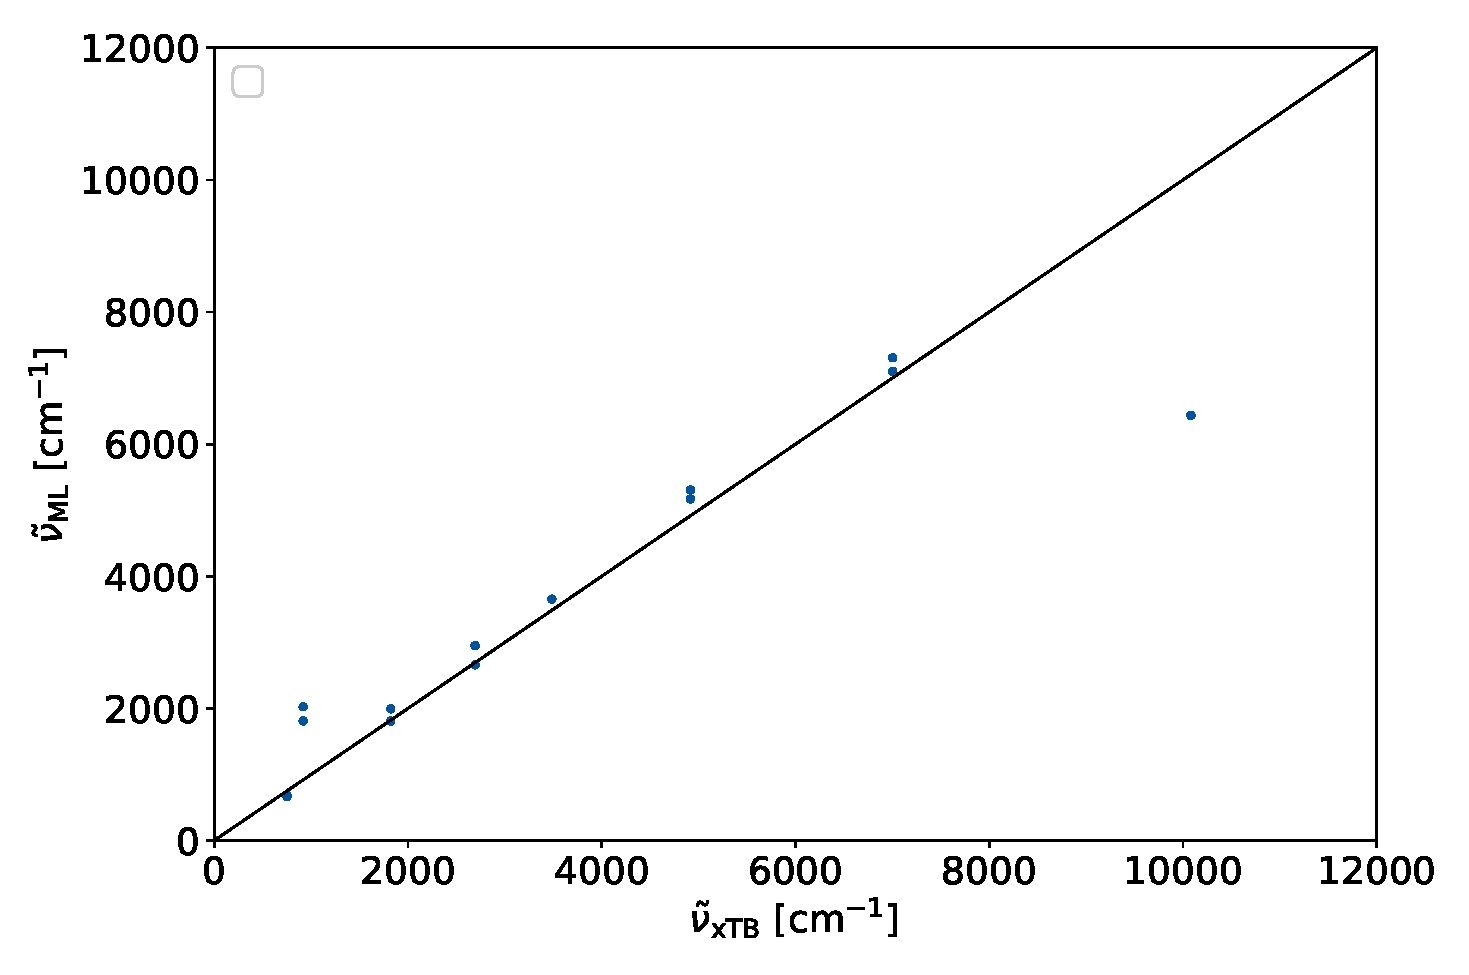
\includegraphics[width = \textwidth]{H2_single/Clean.eps}
    \caption[Plot of wavenumber from GFN2--xTB against wavenumber predicted by a ML model.]{ The wavenumber, predicted via the ML model $\tilde{\nu}_\mathrm{ML}$
    is plotted against the wavenumber calculated via GFN2--xTB $\tilde{\nu}_\mathrm{xTB}$.
    The model uses the Extra Tree Regression.
    The sample set is $\mathrm{H}_2$ and the training set is 75~\% of the whole set.
    The prediction were done for 5 random states.}
    \label{fig:WN_H2}
\end{figure}

\section{Comparison of RFR and ETF}
For the ML models two different algorithms were used, which are the ETR and RFR.
These models are compared to each other by testing there dependency on the amount of training set used.
As the quantity for testing the performance the MSE 
between the predicted hessian and the hessian computed via GFN2--xTB is used.\\
It is expected, that the performance of the ML model should increase, the more data it is trained with. 
To verify this behavior, the training set was increased successively.
The full training set is 75~\% of the full data set. Thus, test set is 25~\%.
While keeping the test set constant, the training set is changed successively between 7.5~\% of the data set to 75~\%.
The MSE was calculated for ten different random states and the mean of these MSE was calculated.
Fig~\ref{fig:Comparison_RFR_ETR} shows the MSE in the dependency of the amount of training set used for the ETR (on the left)
and the RFR (on the right). The error bars indicate the standard deviation.
\begin{figure}[H]
    \centering
    \subfloat{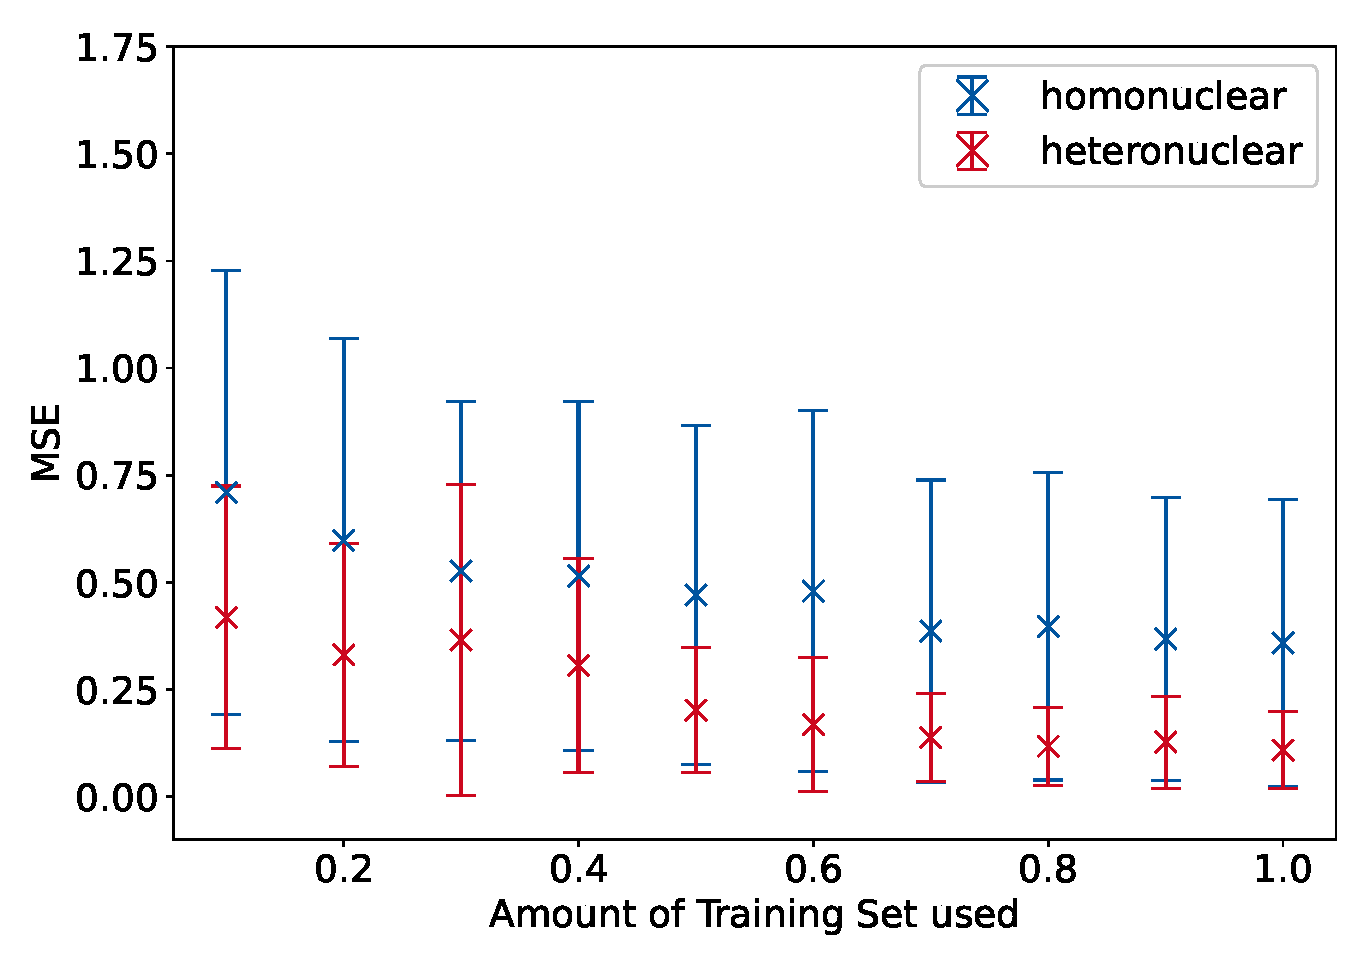
\includegraphics[width = 0.5\textwidth ]{MSE/MSE_ETR.eps}}
    \hfill
    \subfloat{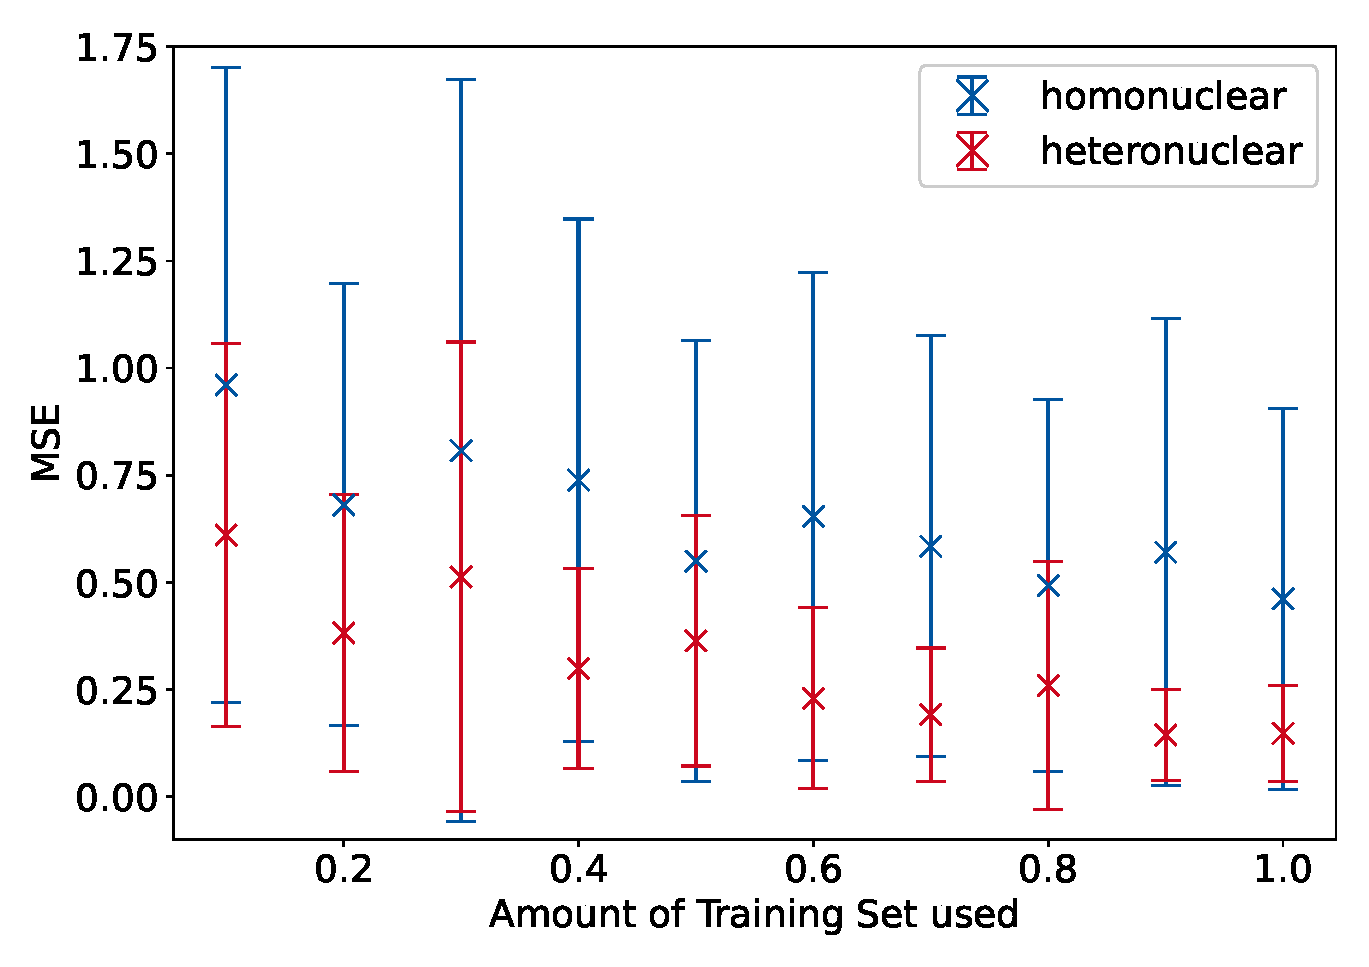
\includegraphics[width = 0.5\textwidth ]{MSE/MSE_RFR.eps}}
    \caption[Learning plots of the ETR and RFR for an increasing size of the training set]{
    Learning plots for the predicting hessian elements~$\frac{\partial^2H}{\partial a \partial b}$
    for an increase of the amount of training set used.
    On the left is the learning plot of the Extra Tree Regression and on the right the plot of the Random Forest Regression shown.
    The full training set is 75~\% of the sample set.
    The full sample set, excluding the $\mathrm{H}_3$~system, is used.
    The mean of ten random states were used for the MSE.
    The plots are done for the homonuclear model (blue) and heteronuclear model (red).}
    \label{fig:Comparison_RFR_ETR}
\end{figure}
In the case of the ETR, the MSE decreases with an increase of the amount of training set used for the homonuclear and heteronuclear model.
This behavior is also recognizable in the case of the RFR.
In comparison to the ETR, the RFR shows a higher standard deviation for the data points.
Thus, the RFR depends more strongly on the random state than the ETR. 
Furthermore, the ETR has, especially for the homonuclear model, lower MSE values for any amount of training set.
At the full amount of training set and at 90\% of the training set,
the RFR and ETR show a similar performance for the heteronuclear model.
All in all, the ETR shows a better performance for the whole investigated range.\\
There is the possibility, that the ML model has so much information in the features,
that it can always predict the target. Hence, the model is tested on whether this is the case,
or the ML model learns from the information of the feature.
For this, the features are scattered with a random factor.
The intensity of the scattering is amplified by the factor $\sigma$.
It is expected, that a model that learns from the features performs worse,
if the scattering of the data points increases.
\begin{figure}[H]
    \centering
    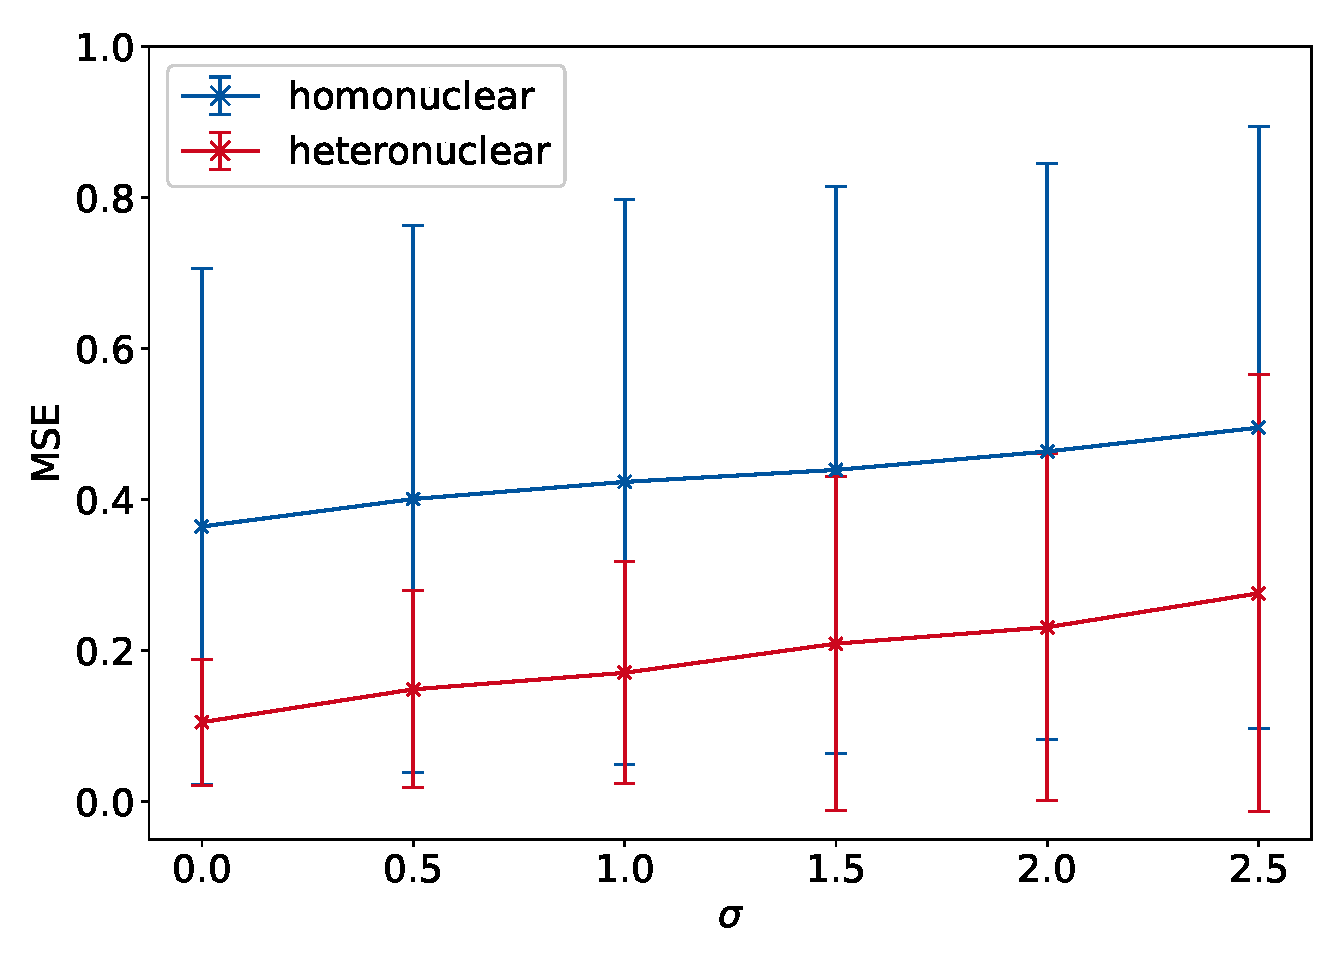
\includegraphics[width = \textwidth]{MSE/MSE_vs_sigma.eps}
    \caption[Learning plot for hessian elements with an increase of randomness on $\textbf{x}$]{
    Learning plots for predicting hessian elements~$\frac{\partial^2H}{\partial a \partial b}$
    for a variation of the factor~$\sigma$.
    The full sample set, excluding the $\mathrm{H}_3$~system, is used for the Ml models.
    The mean of ten random states were used for the MSE.
    The plots are done for the homonuclear model (blue) and heteronuclear model (red).}
    \label{fig:MSE_sigma}
\end{figure}
The performance of the model ETR--Multi--Permuted was tested for this. 
The prediction was done for ten different random states.
The MSE between the predicted hessian elements and the via GFN2--xTB calculated ones was investigated.
For the investigated range of $0 \leq \sigma \leq 2.5$ the MSE increases monotonically.
Hence, this shows, that the model learns from the features and is not purely random.\\
In this section a comparison of the RFR and ETR was done.
The ETR shows overall a better performance than the RFR.
Furthermore, it could be verified,
that the ML model learns from the features used for the prediction of the hessian matrices.


\section{Comparison of Permutation Model and Indexed Model}
Beside the different algorithms for the construction of the trees, other model changes were done.
These differences are investigated in this section. On the one hand,
a multimolecule model was constructed as also several single molecules.
On the other hand, it can be differentiated between the indexed and permuted model.
For the investigations in this section, 
the difference between the prediction and GFN2--xTB calculation were computed.
From these differences the standard deviation as also the mean were calculated,
and a Gaussian distribution was assumed.
This was done for the models ETR--Perm--Multi, ETR--Perm--Single, ETR--Idx--Multi and ETR--Idx--Single.\\
At first the direct prediction of the hessian elements were investigated.
Fig.~\ref{fig:ErrorDistHess} shows the distribution for the prediction of the hessian elements.

\begin{figure}[H]
    \centering
    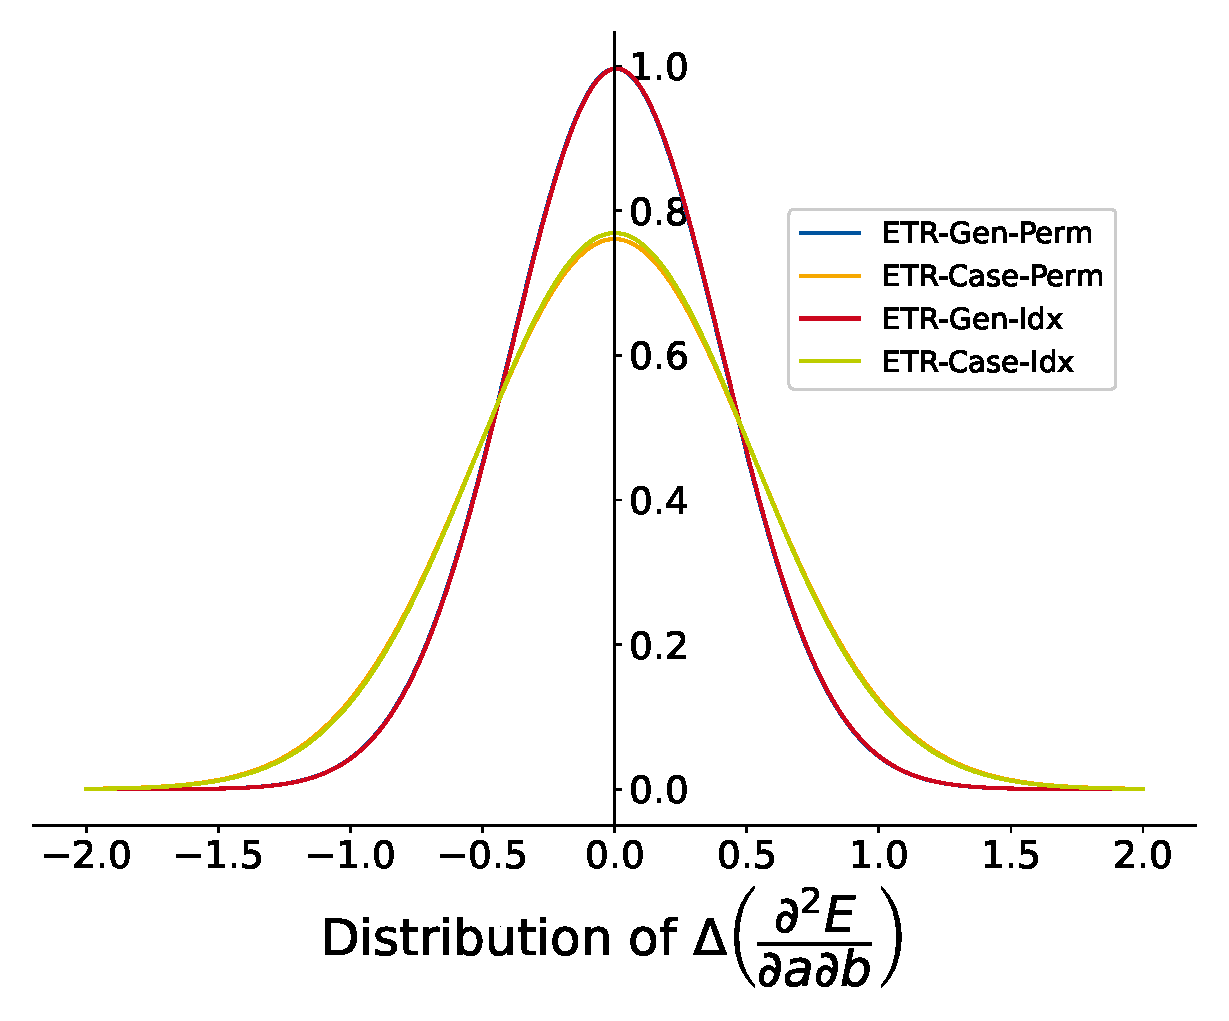
\includegraphics[width = \textwidth]{ErrorDistGraphs/error_distribution_ml_hess.eps}
    \caption[Gaussian type distribution for the prediction of hessian elements.]{ Distribution of $\Delta \left(\frac{\partial^2 E}{\partial a \partial b}\right)$ for different models.
    In every model, the Extra Tree Regression was used.
    The distribution is assumed to be Gaussian type.
    For this the median and standard deviation of $\Delta \left(\frac{\partial^2 E}{\partial a \partial b}\right)$ are computed. }
    \label{fig:ErrorDistHess}
\end{figure}
Comparing the ETR--Perm--Single and ETR--Idx--Single as also ETR--Perm--Multi and ETR--Idx--Multi shows,
that both approaches for the labeling of the features do not differ significantly.
Thus, both approaches are in good agreement with another.
This shows, on the one hand, the strength of the decision tree algorithms.
They cannot overfit and seem to be capable of describing this complex system with a simple differentiation by indexes.
On the other hand, the permuted model does the same prediction for the model,
but may be useful for other machine learning algorithms or even neural networks.\\
The comparison of the ETR--Perm--Single and ETR--Perm--Multi
shows, that the ETR--Perm--Single model deviates more strongly.
This is in agreement with the comparison of the ETR--Idx--Single and ETR--Idx--Multi models.
Though the deviation is stronger, the means of the models do not differ significantly. 
The data set for training the models is smaller for the Single models than for the Multi models.
This might be the reason for the deviation.\\

\begin{figure}[H]
    \centering
    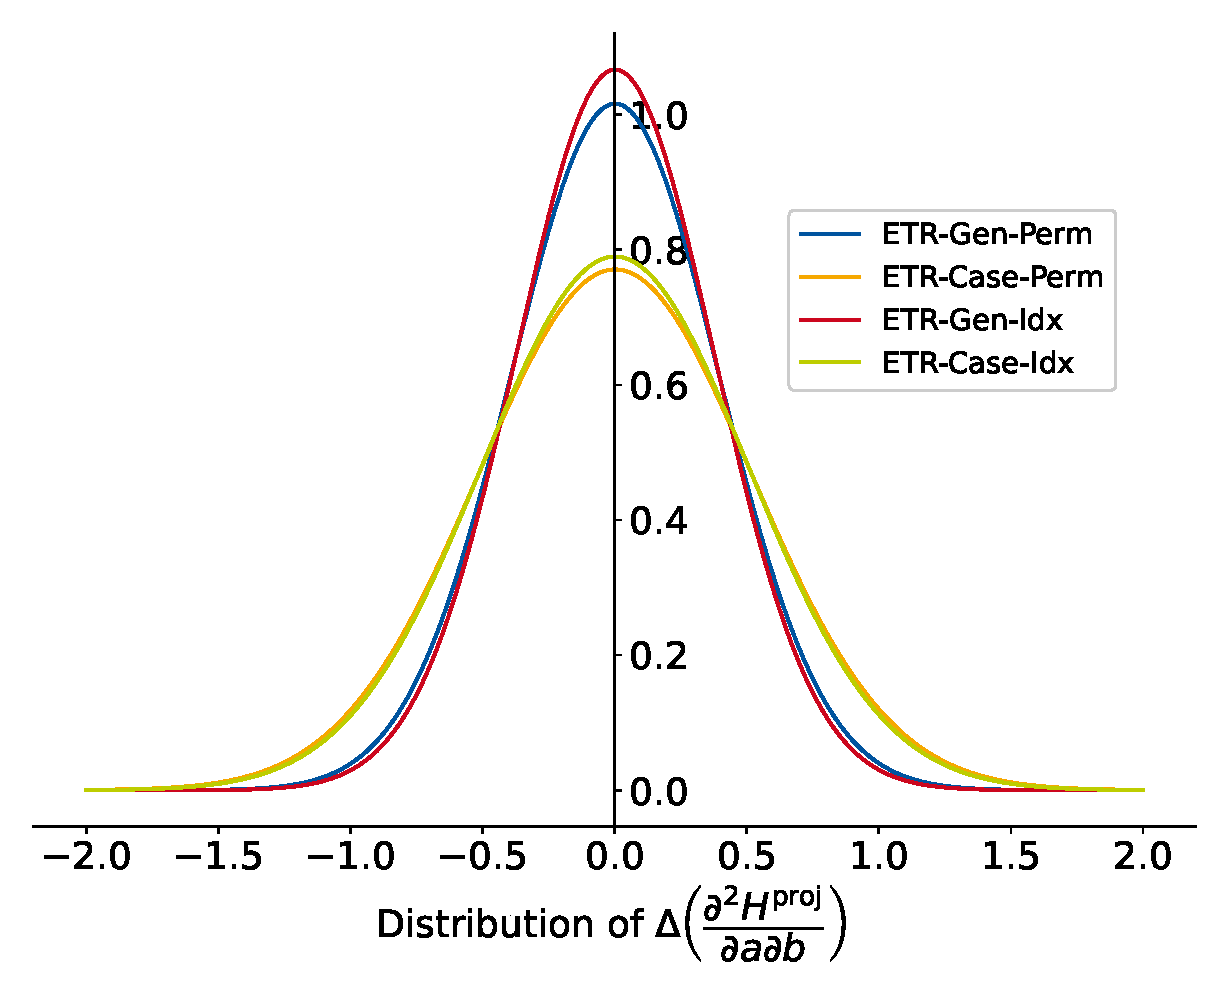
\includegraphics[width = \textwidth]{ErrorDistGraphs/error_distribution_ml_hess_p.eps}
    \caption[Gaussian type distribution for the prediction of projected hessian elements.]{
    Distribution of $\Delta \left(\frac{\partial^2 E^\mathrm{proj}}{\partial a \partial b}\right)$ for different models.
    In every model, the Extra Tree Regression was used.
    The distribution is assumed to be Gaussian type.
    For this the median and standard deviation of $\Delta \left(\frac{\partial^2 E^\mathrm{proj}}{\partial a \partial b}\right)$ are computed. }
    \label{fig:ErrorDistHessP}
\end{figure}

\begin{figure}[H]
    \centering
    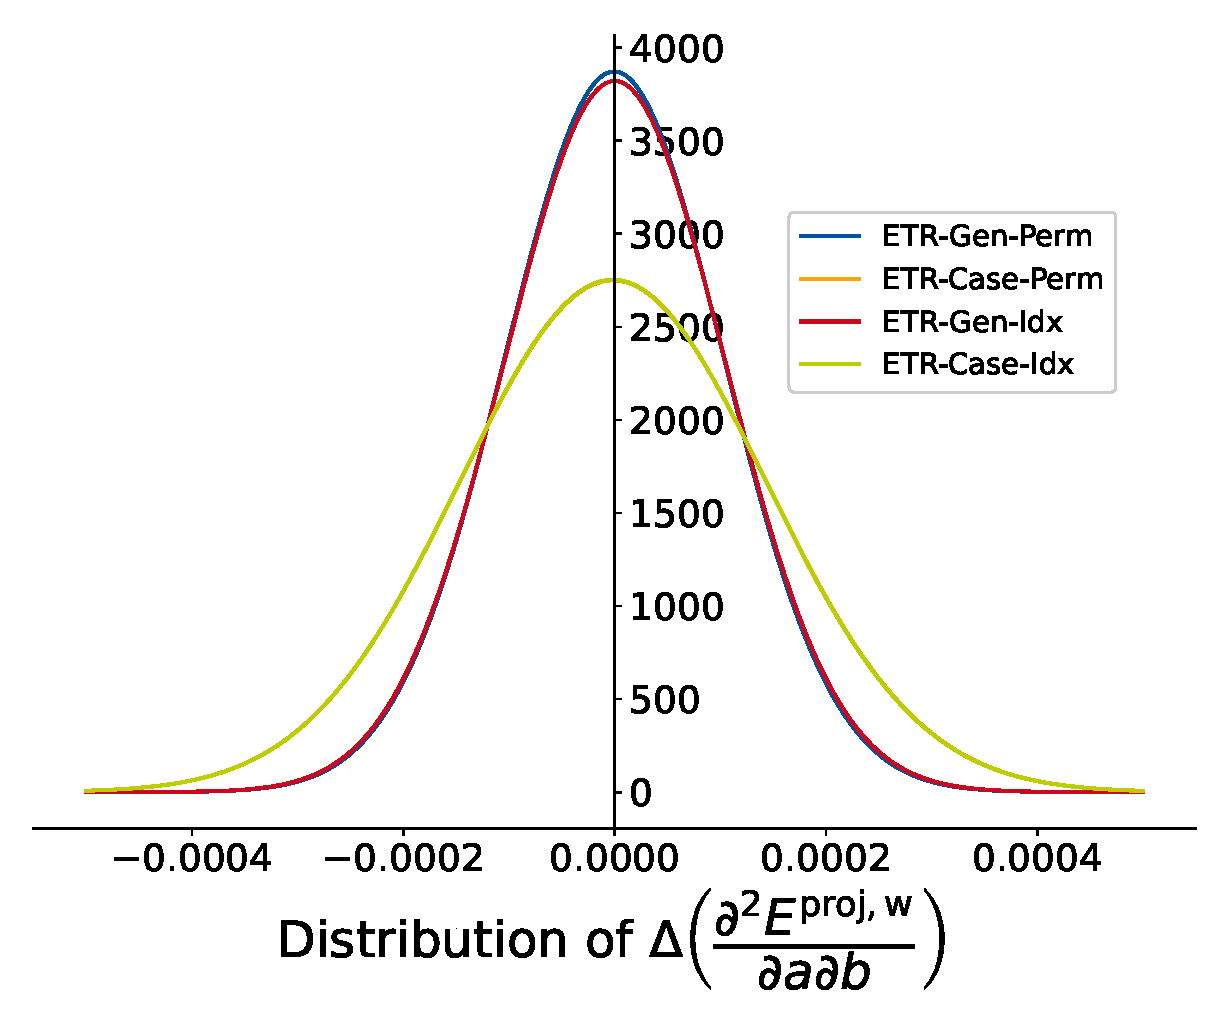
\includegraphics[width = \textwidth]{ErrorDistGraphs/error_distribution_ml_hess_w.eps}
    \caption[Gaussian type distribution for the prediction of weighted projected hessian elements.]{
    Distribution of $\Delta \left(\frac{\partial^2 E^\mathrm{proj,w}}{\partial a \partial b}\right)$ for different models.
    In every model, the Extra Tree Regression was used.
    The distribution is assumed to be Gaussian type.
    For this the median and standard deviation of $\Delta \left(\frac{\partial^2 E^\mathrm{proj,w}}{\partial a \partial b}\right)$ are computed. }    \label{fig:ErrorDistHessW}
\end{figure}

\begin{figure}[H]
    \centering
    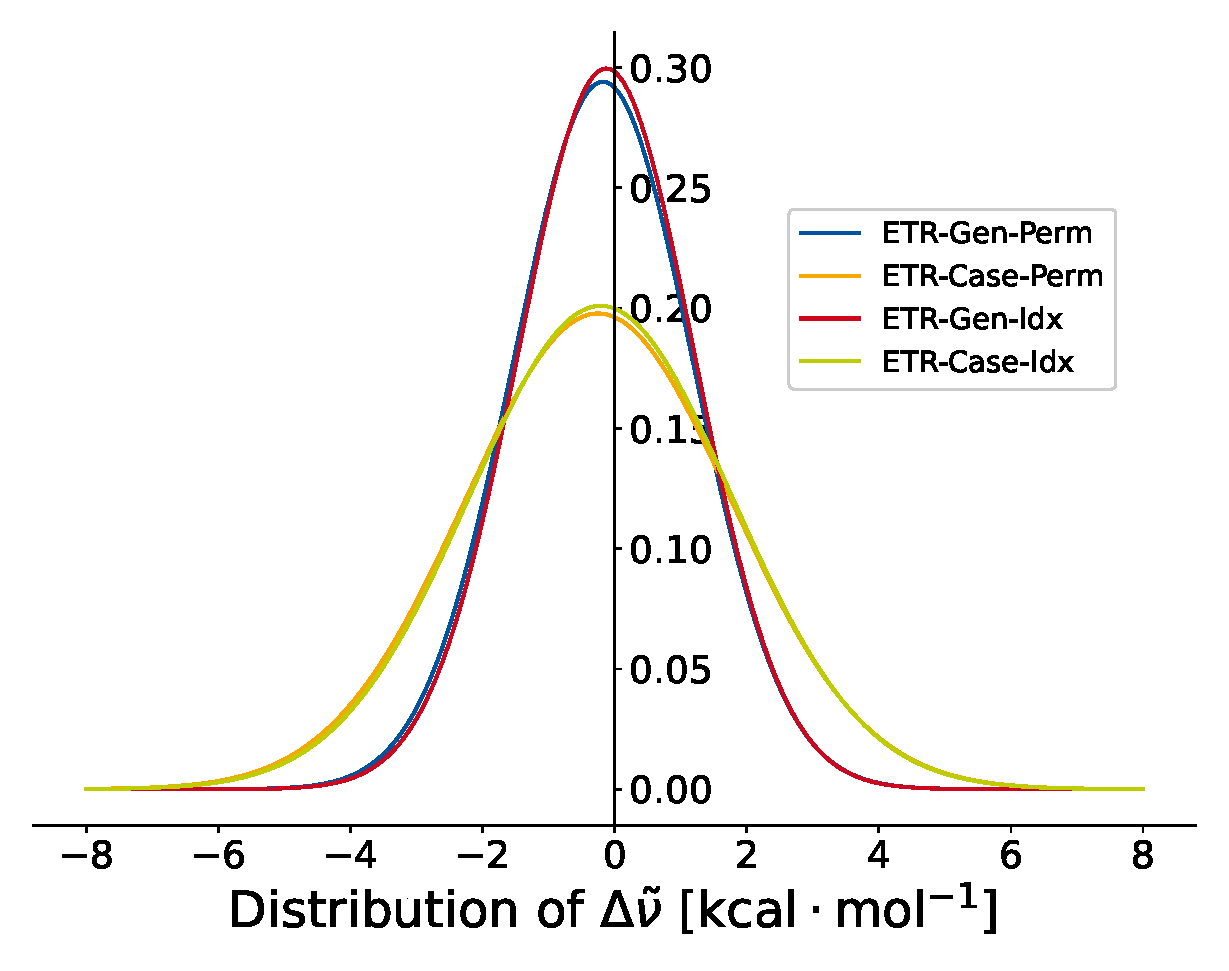
\includegraphics[width = \textwidth]{ErrorDistGraphs/error_distribution_ml_wn.eps}
    \caption[Gaussian type distribution for the prediction of wavenumbers.]{
    Distribution of $\Delta \tilde{\nu}$ for different models.
    In every model, the Extra Tree Regression was used.
    The distribution is assumed to be Gaussian type.
    For this the median and standard deviation of $\Delta \tilde{\nu}$ are computed.}
    \label{fig:ErrorDistWN}
\end{figure}

\begin{figure}[H]
    \centering
    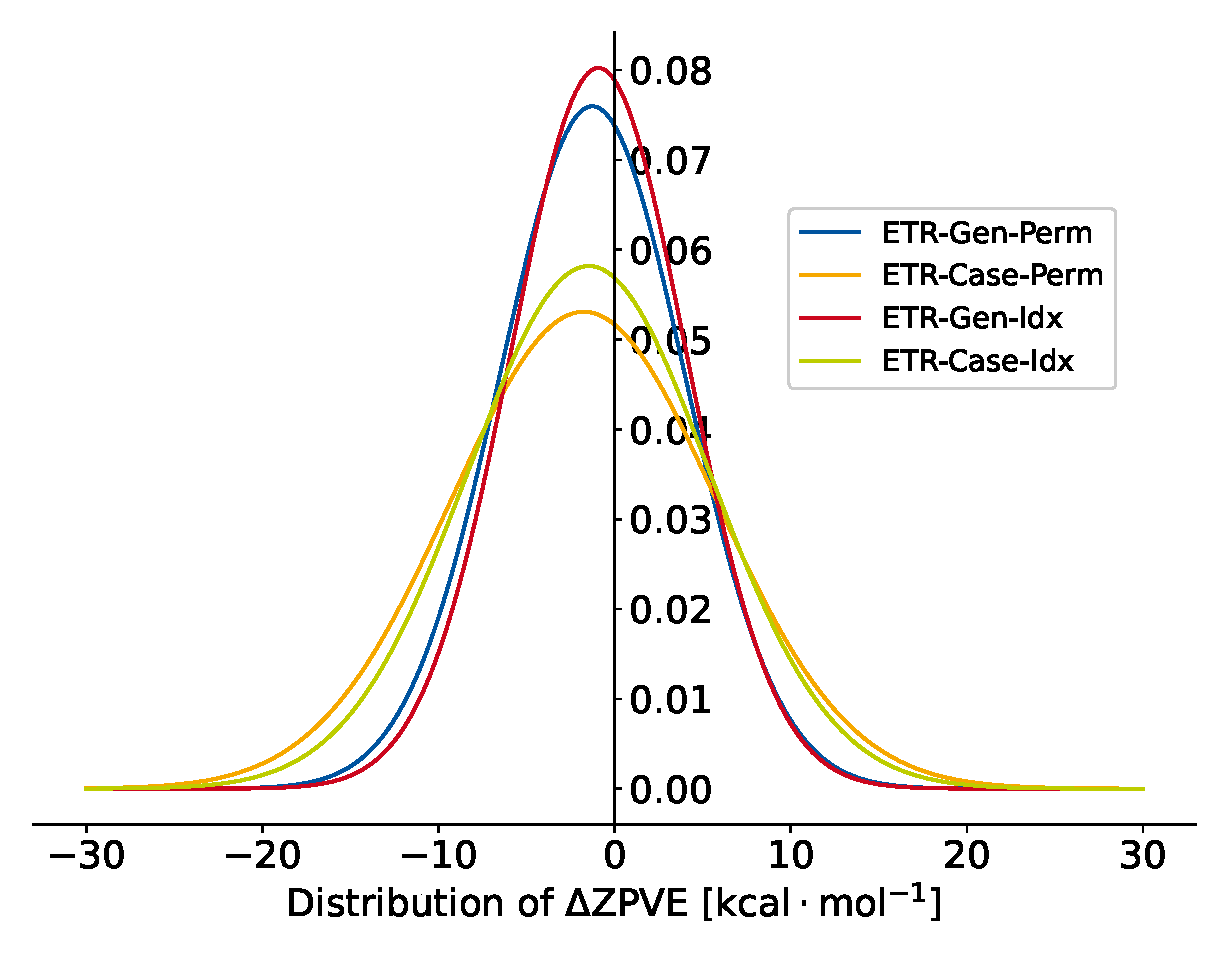
\includegraphics[width = \textwidth]{ErrorDistGraphs/error_distribution_ml_ZPE.eps}
    \caption[Gaussian type distribution for the prediction of zero point energy.]
    {Distribution of $\Delta \mathrm{ZPE}$ for different models.
    In every model, the Extra Tree Regression was used.
    The distribution is assumed to be Gaussian type.
    For this the median and standard deviation of $\Delta \mathrm{ZPE}$ are computed.}
    \label{fig:ErrorDistZPE}
\end{figure}

\section{Benchmarking the H$_\mathrm{\textbf{3}}$~system}
Especially, the prediction of hessian matrices of fully unknown systems is of interest.
Hence, the ETR-Gen-Perm and ETR-Gen-Idx models were tested on the performance on a new, for the model unknown, system.
For the $\mathrm{H}_3$ system the outer hydrogen atoms were fixed,
while the hydrogen atom was shift from one hydrogen to another.
For each position of the hydrogen atom,
the force constants of the systems were predict via the ML model.
The force constants were also calculated via GFN2--xTB.\\
Fig.~\ref{fig:FC_idx} shows the force constants calculated by GFN2--xTB and predicted via the ETR--Gen--Idx model.
Interesting to point out is the symmetric behavior of the system.
The ML model should, in principle, mimic this behavior.
While this is overall the case, there are abbreviation from this behavior.
For the example, the symmetry is not given in the case of $x(\mathrm{H2}) = 1.75$ and $x(\mathrm{H2} = 2.25)$.
\begin{figure}[H]
    \centering
    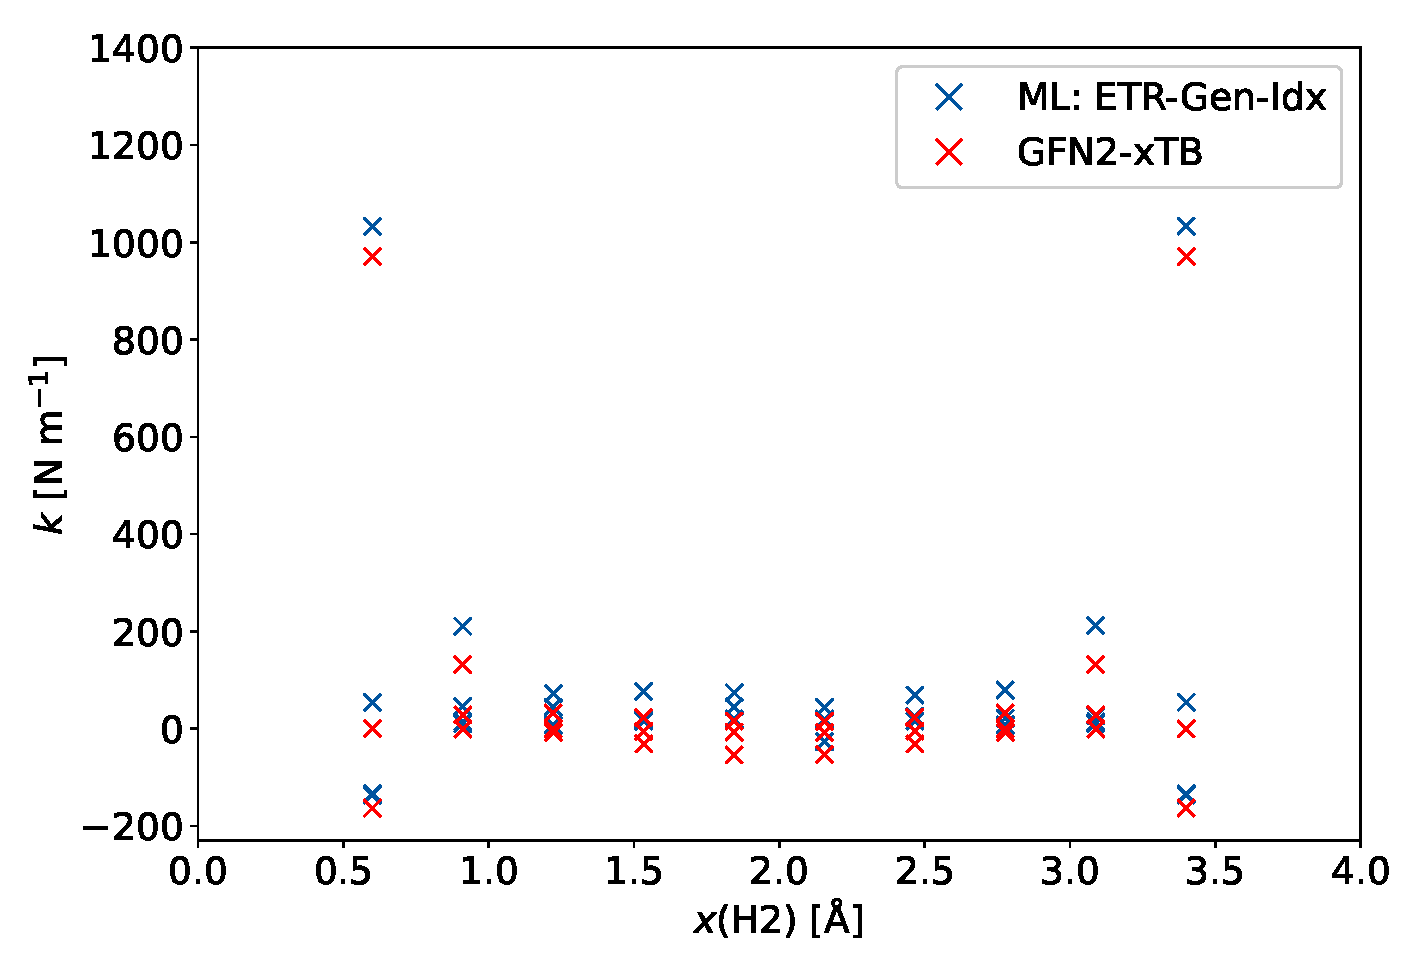
\includegraphics[width = \textwidth]{ForceConstants/force_const_H3_idx.eps}
    \caption[Force constants predicted by the indexed multimodel and calculated with
    GFN2--xTB for $\mathrm{H}_3$~system]{
    Force constants predicted for the $\mathrm{H}_3$~systems in dependence of the distance between H1 and H2 are shown.
    The force constants are shown for the GFN2--xTB calculation (yellow),
    as also the via the ML model predicted values (blue).
    The full sample set, excluding the $\mathrm{H}_3$~system, was used for the ML model.
    The ML model \textit{indexed; multi} was used for the prediction.
    }
    \label{fig:FC_idx}
\end{figure}

\begin{figure}[H]
    \centering
    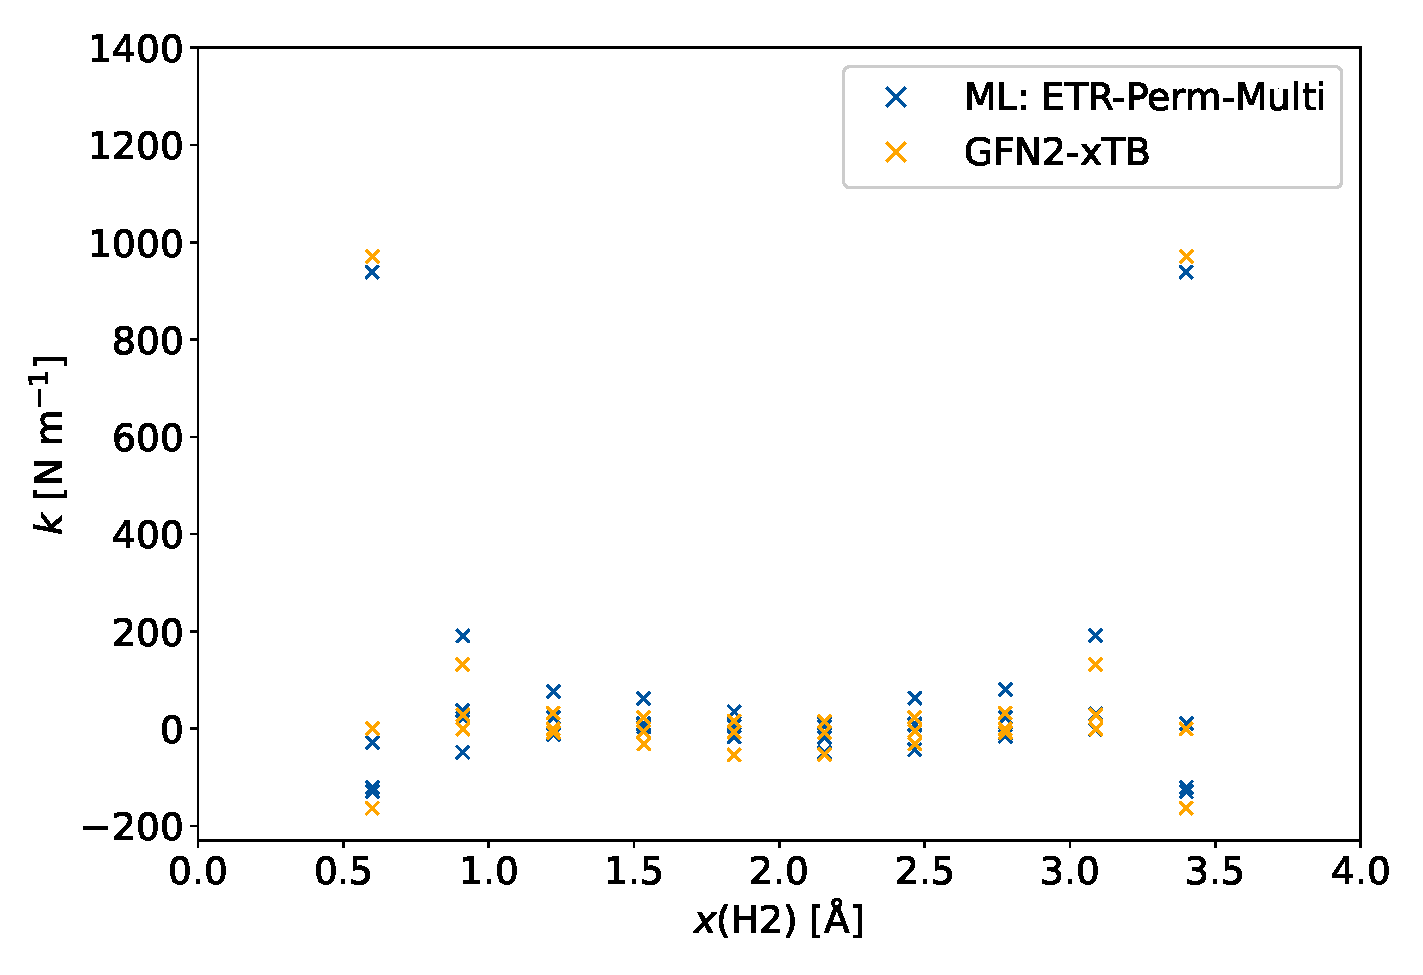
\includegraphics[width = \textwidth]{ForceConstants/force_const_H3_perm.eps}
    \caption[Force constants predicted by the permuted multimodel and calculated with
    GFN2--xTB for $\mathrm{H}_3$~system]{Force constants predicted for the $\mathrm{H}_3$~systems in dependence of the distance between H1 and H2 are shown.
    The force constants are shown for the GFN2--xTB calculation (yellow),
    as also the via the ML model predicted values (blue).
    The full sample set, excluding the $\mathrm{H}_3$~system, was used for the ML model.
    The ML model \textit{perm; multi} was used for the prediction.}
    \label{fig:FC_perm}
\end{figure}
